\chapter{Visualisation Evaluation}\label{C:sd}
Following the completion of the implementation stage of this project a final
user evaluation was carried out on the visualisation. This evaluation was
primarily designed to discover whether or not the visualisation created was
successfull in fulfilling the requriemnts of the project as well as conveying
the information stored within the Kepler Exoplanet Database.

\section{Why was evaluation conducted}

\section{Expectations of evaluation}

\section{Evaluation Environment}

\section{User Study Method}
\begin{itemize}
\item The user enters the room and sits down at the computer.
\item They are handed the consent form and information sheet.
\item After these are completed they are handed the user questionnaire and the
set of questions to answer while using the system. On this questionnaire there
are two sets of questions, the first is for the keyboard and mouse system, and
the second if for the Microsoft Kinect system.
\item Following this they are advised that they have 5 minutes to get
familiarised with the system but they do not need to use all of this time (the
amount of time taken will be recorded for analysis of how user friendly and
intuitive the system is).
\item Following this the user is asked to complete the question sheet by first
using the mouse and keyboard system. When they feel they have answered all of
the questions they will notify the examiner who will move the user to the Kinect
system to continue the questions.
\item Once the user has completed both sets of questions they are asked to fill
in the qualitative user questionnaire about their experiences using the
visualisation. 
\item Following this if the examiner has no follow up questions the user is free
to leave.
\end{itemize}

\subsection{Participants}
The number and demographics of participants in a user study is a key issue that
can affect the results. ~

\section{Pilot Study}
One participant was asked to take part in a pilot study before any results were
collected. This participant was asked to complete all of the activites that make
up the main experiment. This pilot study took approximately 15 minutes as
intended, this included the time needed for the explanation and completion of
paperwork, as well as the experiment itself.

The reason for conducting this pilot study was to ensure that the experiment was
producing the data required to evalutate the the visulaisation produced as well
as taking the correct amount of time to complete. In addition to this it was
used to discover whether there were any aspects of the study that would
interfere with the results.

A result of perfoming this pilot study was that it revealed that the wording of
some of the tasks users were asked to complete were ambiguous and caused
unneccesary confusion for users during the experiment which could have
interfered with the results in a negative way. These ambigous questions and
tasks were removed prior to the main user study. During the main study no users
asked for  clarrification on any of the questions or tasks.

\section{Experiment on Keyboard and mouse visualisation}
Image of using kinect system

\section{Experiment on Microsoft Kinect visualisation}

\section{Results}
The user study was undertaken by 9 participants, all were either students or
young professionals from a mix of specialities aged between 21 to 26 with a mix
of genders with 5 females and 4 males. Each study took between 10 to 15 minutes.


\subsection{Analysis of requirements}
\begin{enumerate}

 \item[R1.] The visualisation needs to display planetary information to convey
knowledge to users.
 \item[R2.] The planets need to be able to be ordered by their similarity to
earth (ESI) and by their Kepler Object of Interest number (KOI).
 \item[R3.] The visualisation needs to allow users to define ranges of planetary
attributes to filter which planets are displayed.
 \item[R4.] All planets need to be selectable and react appropriately when
clicked.
 \item[R5.] When a planet is selected all other planets in the same solar system
need to become more visible.
 \item[R6.] There needs to be the option to view the habitable zones of stars
and show where the planets orbiting them are in relation.
 \item[R7.] The visualisation needs to allow exoplanets to be compared against
one another.
\end{enumerate}

 The non functional requirements for this visualisation are as follows:
\begin{enumerate}
 \item[R8.] The visualisation needs to have a range of interactive buttons for
each element of interactivity in the system to help inform users how to use the
system.
 \item[R9.] All interaction methods must be visible and intuitive.
 \item[R10.] The visualisation needs to display attributes of each of the
Exoplanets.
 \item[R11.] The visualisation must remain uncluttered.
 \item[R12.] The visualisation must not show so much information that it causes
information overload for users.
  \item[R13.] There needs to be two modes of interaction with the system,
keyboard and mouse vs gesture based.
\end{enumerate}

Image of using non kinect system
\begin{figure}[h!]
  \centering
      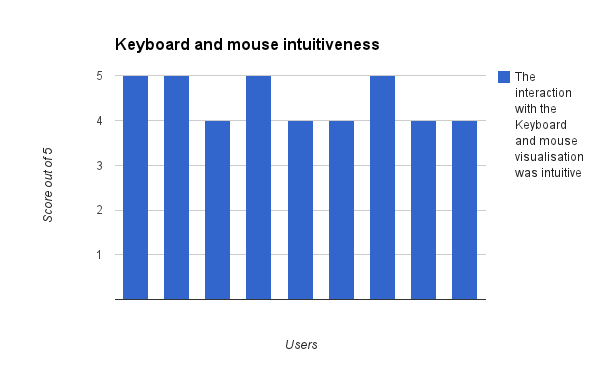
\includegraphics[width=0.8\textwidth]{images/charts/chart_1.png}
  \caption{Intuitivity of keyboard and mouse}  
    \label{fig:chart1}
      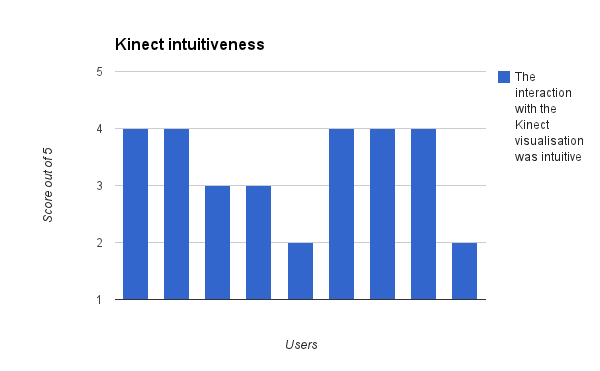
\includegraphics[width=0.8\textwidth]{images/charts/chart_2.png}
  \caption{Intuitivity Microsoft Kinect sensor}  
    \label{fig:chart2}
      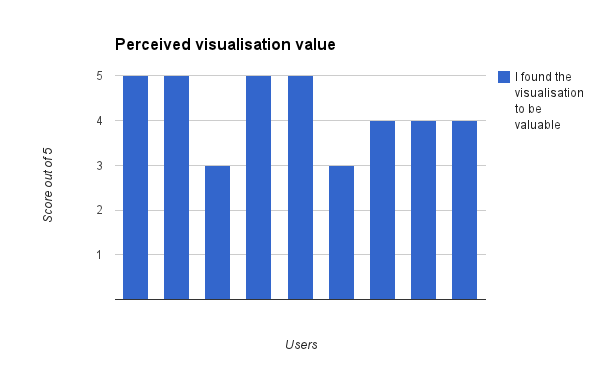
\includegraphics[width=0.8\textwidth]{images/charts/chart_3.png}
  \caption{Perceived value of visualisation}  
    \label{fig:chart3}
\end{figure}

\begin{figure}[h!]
  \centering
      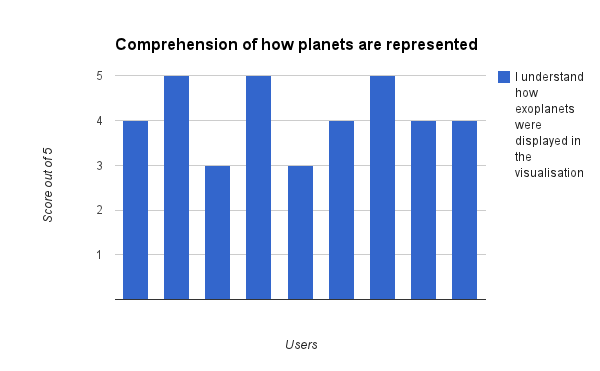
\includegraphics[width=0.8\textwidth]{images/charts/chart_4.png}
  \caption{User comprehension of visualisation}  
    \label{fig:chart4}
      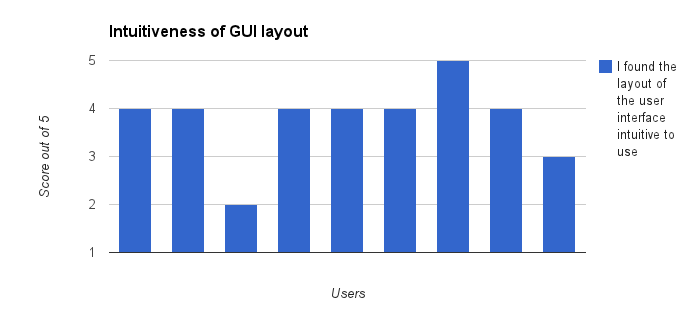
\includegraphics[width=0.8\textwidth]{images/charts/chart_5.png}
  \caption{GUI layout intuitivity}  
    \label{fig:chart5}
\end{figure}

\begin{figure}[h!]
  \centering
      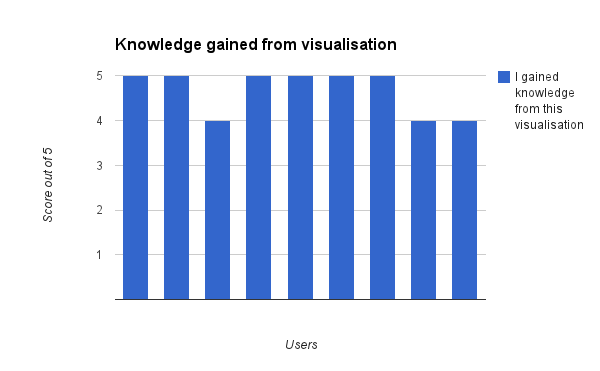
\includegraphics[width=0.8\textwidth]{images/charts/chart_7.png}
  \caption{Knowledge gained from the visualisation}  
    \label{fig:chart7}

      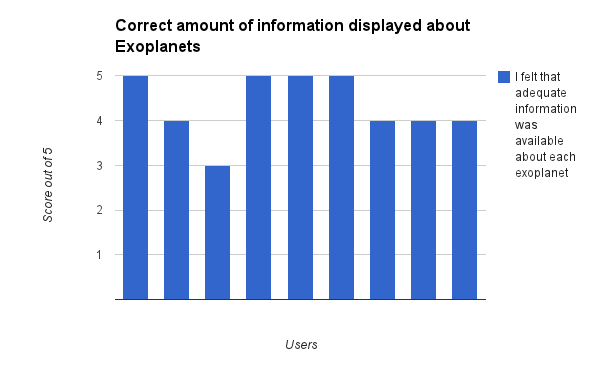
\includegraphics[width=0.8\textwidth]{images/charts/chart_8.png}
  \caption{Correct amount of information displayed}  
    \label{fig:chart8}
      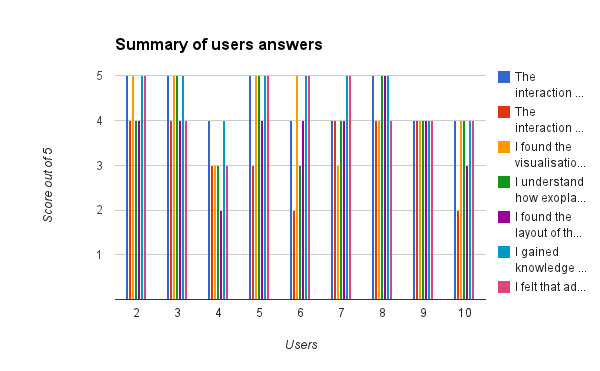
\includegraphics[width=0.8\textwidth]{images/charts/chart_9.png}
  \caption{Summary of results}  
    \label{fig:chart9}
    
\end{figure}
\section{Threats to validity}
